\documentclass[11pt,letterpaper,english]{article}
\usepackage[T1]{fontenc}
\usepackage[latin1]{inputenc}
\setlength\parskip{\medskipamount}
\setlength\parindent{0pt}
\usepackage{amsmath}
\usepackage{graphicx}
\usepackage{amssymb}
\usepackage{babel}
%use epsfig package for figs
\usepackage{epsfig}
\makeatother
\usepackage{multirow}

%%\usepackage[scaled=0.92]{helvet}
\usepackage{helvet}
\usepackage[sf]{titlesec}
\renewcommand\familydefault{\sfdefault}
\usepackage{url}

%use lgrind to include code listing
%\usepackage{lgrind}

%other formatting stuff
\oddsidemargin 0pt
\flushbottom
\parskip 10pt
\parindent 0pt
\textwidth 465pt
\topmargin 10pt
\textheight 610pt
\renewcommand{\baselinestretch}{1.0}


\begin{document}

% SOME MACROS
\newcommand{\etal}{{\em et al.}}
\newcommand{\ux}{{\underline{x}}}
\newcommand{\tdt}{{t}} 

{\bf {\large A1. CARIACO model description}} 

NPZD models are simplified marine ecosystem models that can be adapted to different physical settings and food web structures. For this model, the basic structure is inspired by the models of Fasham (1990) as it was adapted by Anderson et al. (2015). The pyhsical setting of the model uses a zero-dimensional slab structure as originally presented in Evans and Parslow (1985) and adapted from Acevedo-Trejos et al. (2015) where the ecosystem is described within a seasonally varying surface mixed layer above a deep homogenous layer. The code structure is the PhytoMFTM model written in the open source programming language Python, which provides a flexible framework for NPZD-type models with multiple functional types of phytoplankton and zooplankton. The model code and all statistical scripts are available publicly on Github (\url{https://github.com/ben1post/BennyPhD}).

The model framework was adapted to the setting of the CARIACO time-series at $10.5°$ N, $64.67°$ W in the Cariaco basin of the coast of Venezuela. The data includes phytoplankton species counts and two size-classes of zooplankton, which were included in the model as the 4 most prominent phytoplankton types, and 2 zooplankton types. The phytoplankton types include Nanoflagellates $P_{n}$, Diatoms $P_{dt}$, Coccolithophores, $P_{c}$ and Dinoflagellates $P_{dn}$. There are two Zooplankton types split by size class, named Mikrozooplankton $Z_{\mu}$ and Mesozooplankton $Z_{\lambda}$. 
\begin{figure}[b!]
\centering
  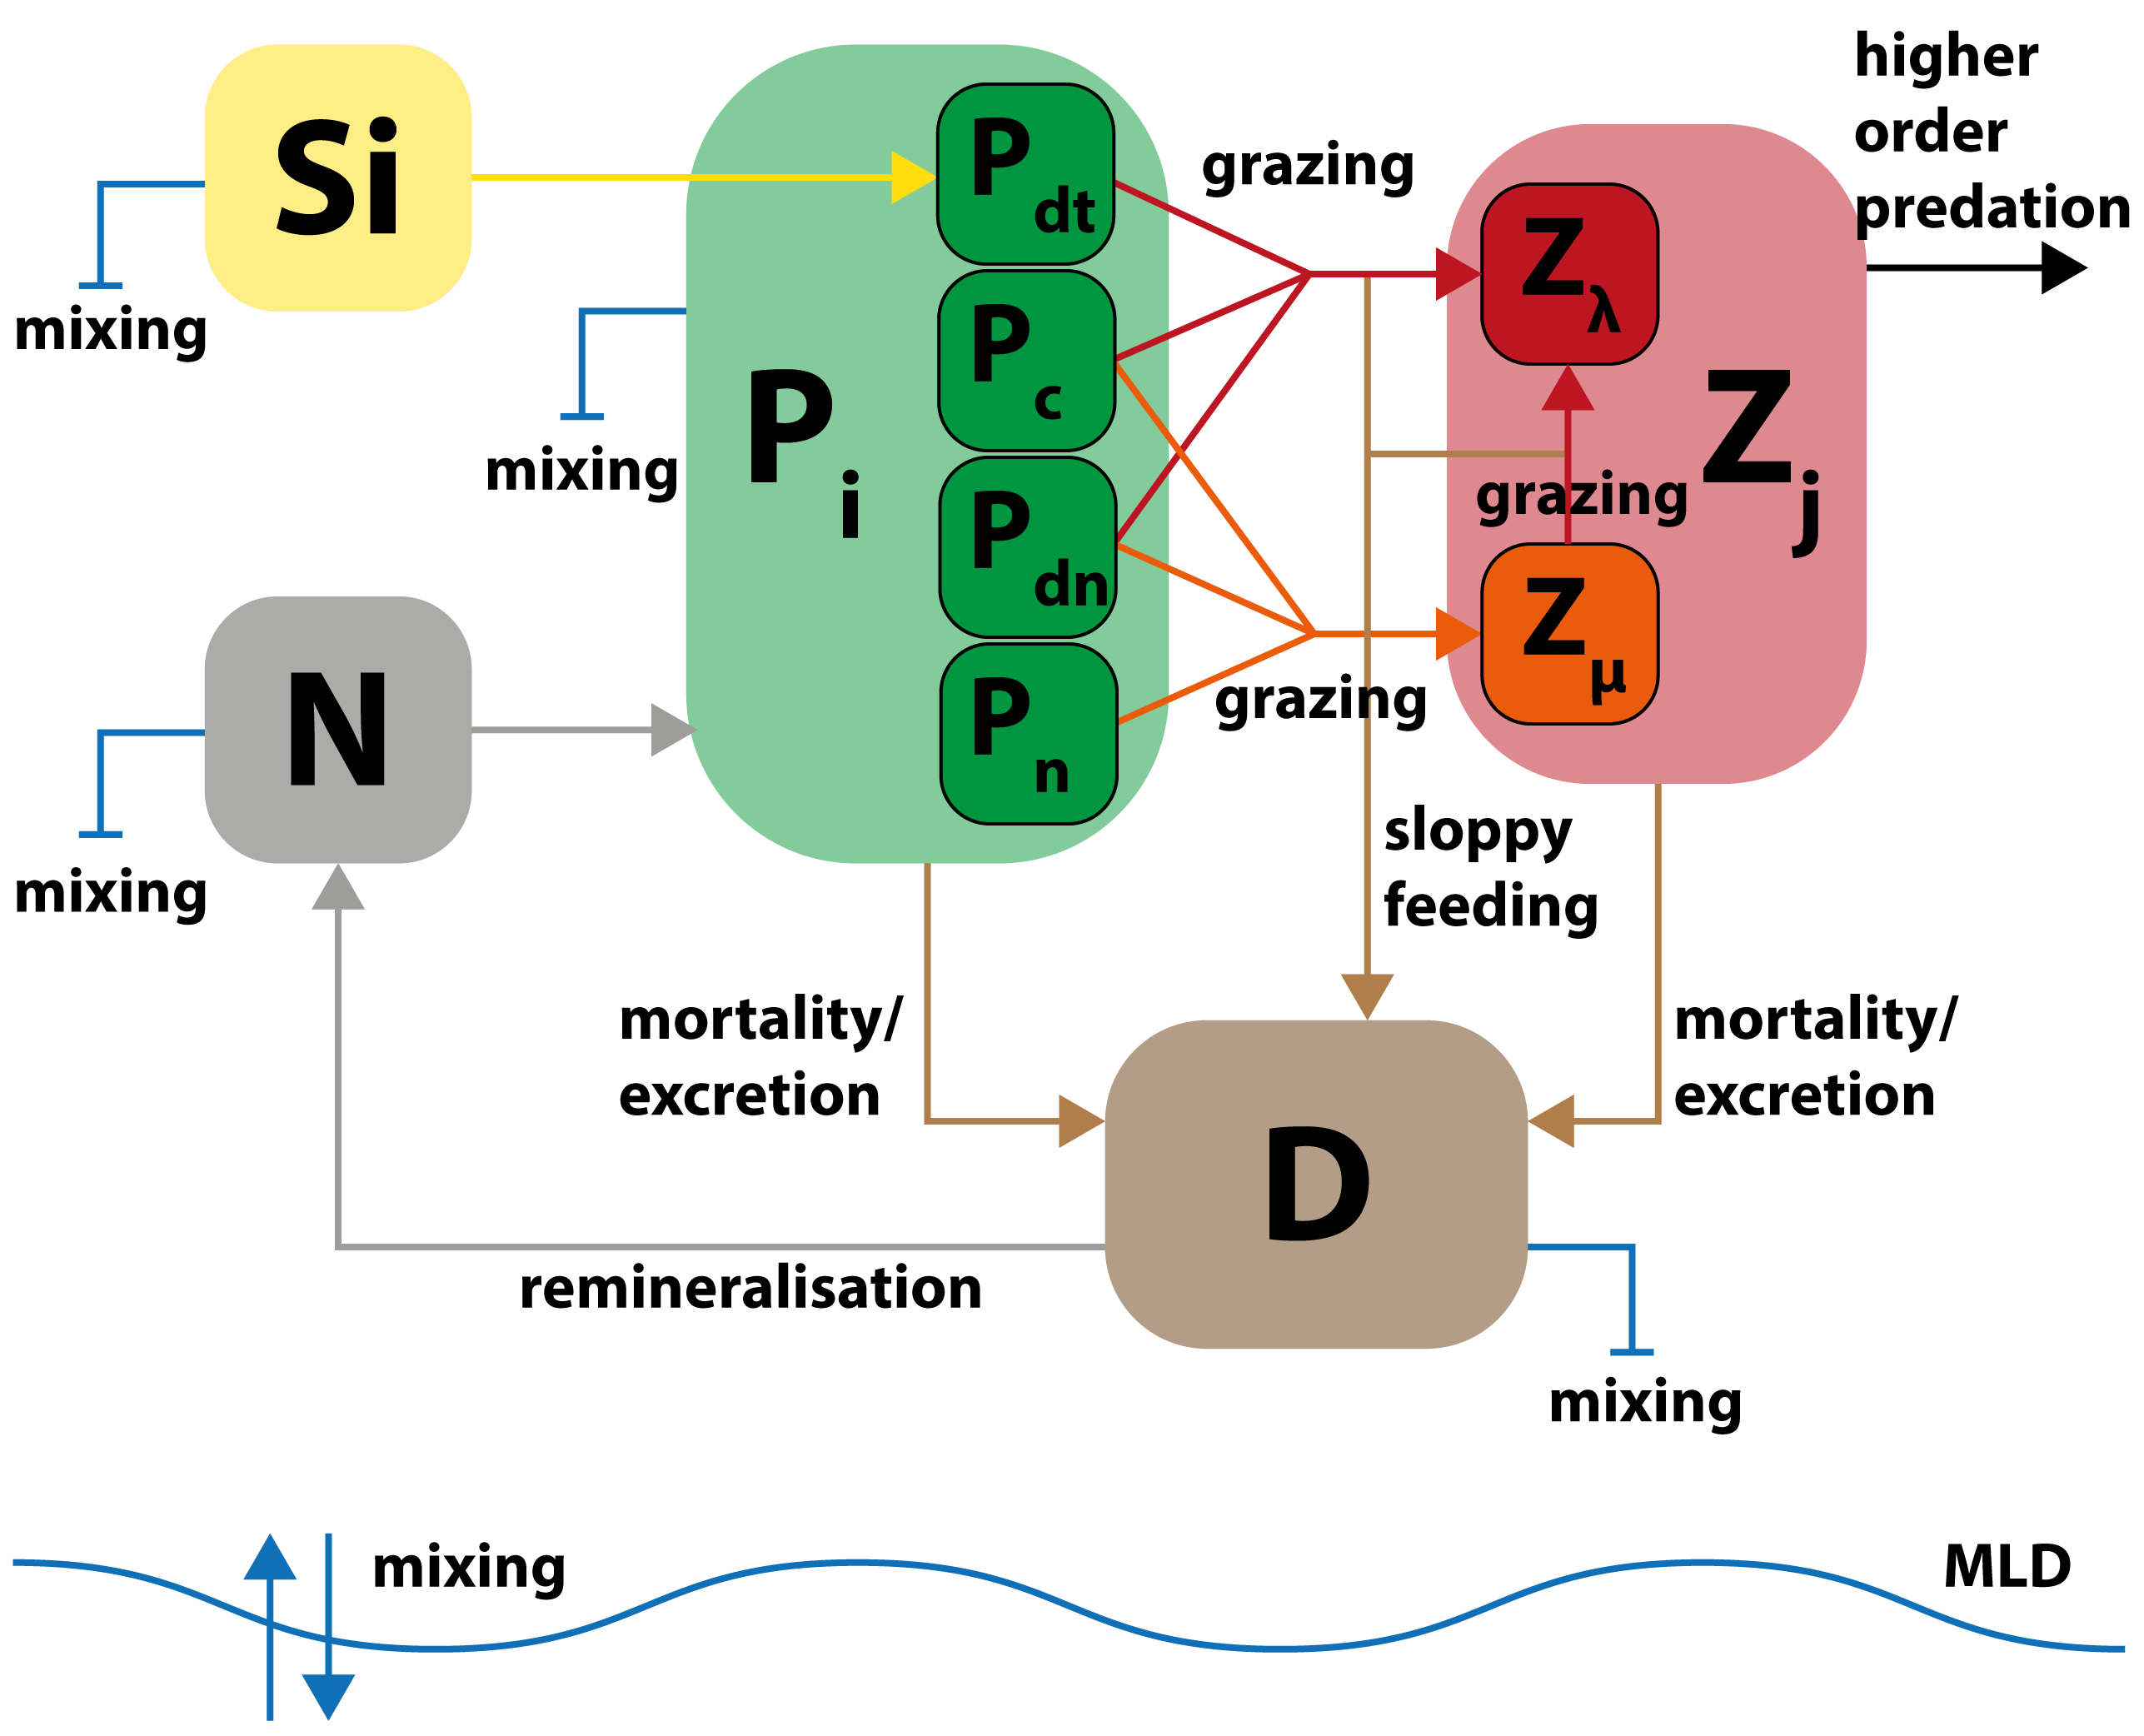
\includegraphics[width=0.7\linewidth]{images/whiteArtboard4ModelSchematics.png}
  \caption{Model schematics of CARIACO model.}
  \label{fig:boat1}
\end{figure}
Nitrogen $N$ (and Silicate $Si$ for Diatoms) is assimilated by the phytoplankton types $P_i$, which are grazed by the zooplankton types $Z_j$. Mortality of and excretion from phytoplankton and zooplankton, and sloppy feeding by zooplankton contribute to Detritus $D$. In addition to the linear mortality of $P_i$ and $Z_j$, there is an additional quadratic mortality term acting on $Z_j$, which represents higher-order predation on zooplankton.

{\bf {\large A1.1 Physical setting}}

The ecosystem component of the model is set within a zero-dimensional physical environment. The water column is divided into a 2-layer structure. A depth variable layer (e.g. the thermo- and/or pycnocline) separates a well-mixed surface layer containing the ecosystem component from a homogenous deep ocean. Concentrations of nutrients are averaged across the mixed layer, and remain constant below.  There is no lateral advection, but vertical mixing is modeled as a function of mixed layer depth (MLD) over time $M(t)$. Temperature depth profiles have been used to reconstruct the MLD at the investigated location. The derivative of MLD over time is given as $h(t) = dM(t)$. Exchange between the two layers is described by the two processes of turbulent diffusion and entrainment or detrainment caused by a shallowing or deepening of MLD. Adapted from Fasham (1993), the effects of entrainment and detrainment on nutrients, phytoplankton and detritus are given by the term $h^{+}(t)= max[h(t),0]$. Zooplankton is assumed to be able to maintain themselves within the mixed layer depth, therefore entrainment and detrainment of $Z_j$ are described by $h(t)$. Diffusive mixing between the layers has been parameterized with a constant factor $k$. The entire diffusion term is thus
\begin{equation}
\kappa = \frac{k + h^{+}(t)}{M(t)}
\end{equation}
In addition to the MLD interpolated from time series data, the model is externally forced with sea surface temperature (SST) taken from in situ data and interpolated from monthly to daily values and photosynthetically active radiation (PAR) from 8-day averaged SeaWIFs satellite data.

{\bf {\large A1.2 Phytoplankton}}

Phytoplankton growth is a function of light (PAR), temperature (SST) and nutrients. These factors are assumed to independently limit growth, so that (exemplary for $P_{d}$, i.e. diatoms) the growth term is
\begin{equation}
\mu_{d} = \mu_{d}^{max} \cdot U_{d}(N,Si)\cdot L_{d}(PAR)\cdot T_{d}(SST)
\end{equation}
where $\mu_{d}$ is the maximum growth rate per day and $T(PAR)$ is Eppley's formulation for temperature dependent growth (Eppley, 1972), given as $T(SST) = e^{0.063 * SST}$ with temperature in $°C$. The light-limiting term $L(PAR)$ represents the integrated photosynthesis within the mixed layer as a function of incident irradiance at the surface $I_0$. Light attenuation is calculated using the Lambert-Beer law with irradiance at depth $z$ equal to
\begin{equation}
I(z) = I_0 \cdot e^{-k_{PAR} \cdot z}
\end{equation}
Here, $k_{PAR}$ is calculated as the sum of the constant attenuation coefficient of water $k_w$ and the self-shading of phytoplankton $k_c$ with the unit $µM^{-1}$ multiplied by total phytoplankton biomass $P$, i.e. $k_{PAR} = k_w + k_c P$. This model uses the Smith PI curve as a basis for the calculation, with $V_P$ representing the photosynthetic rate, $\alpha$, the initial slope of the PI curve and $V_p^{Max}$, the maximum photosynthetic rate
\begin{equation}
V_p = \frac{\alpha \cdot I \cdot V_p^{Max}} {\sqrt{(V_p^{Max})^2 + \alpha^2 \cdot I^2}}
\end{equation}
Combining equation (2) and (3) as presented in Anderson et al. (2015), the integrated photosynthesis $\bar{V}_p$ over depth $z$ is calculated as
\begin{equation}
\bar{V}_p(z) = \frac{V_p^{Max}}{k_{PAR} \cdot z} \cdot \ln \Bigg( \frac{\alpha \cdot I_0 + \sqrt{(V_p^{Max})^2+(\alpha \cdot I_0)^2}} {\alpha \cdot I(z) + \sqrt{(V_p^{Max})^2+(\alpha \cdot I(z))^2}} \Bigg)
\end{equation}
where $\bar{V}_p$ equals the light-limiting term $L$ in the growth equation (2).

Nutrient limited growth of the phytoplankton community is described via a Monod equation. 
\begin{equation}
U(N) = \frac{N} {k_N + N}
\end{equation}
For diatoms $P_d$ the nutrient limiting term depends on both nitrogen and silicate concentration within the upper layer. According to Liebig's law of the minimum, always the lower nutrient availability limits Diatom growth:
\begin{equation}
U_{d}(N,Si) = min \Big( \frac{N} {k_{d}^N + N}, \frac{Si} {k_{d}^{Si} + Si} \Big)
\end{equation}
All other phytoplankton types are nutrient-limited only by available Nitrogen as in equation (6). Phytoplankton mortality and excretion are parameterized as a linear constant rate $mo$. With $G_{\mu}$ as grazing by Microzooplankton and $G_{\lambda}$ as grazing by Mesozooplankton (defined below), the equations for all phytoplankton types $P_i$ can now be written as
\begin{equation}
\frac{dP_{i}}{dt} = \mu_{i} \cdot P_{i} - mo_{i} \cdot P - G_{\mu}(P_{i}) - G_{\lambda}(P_{i}) - \kappa \cdot P_{i}
\end{equation}

{\bf {\large A1.3 Zooplankton}}

Two zooplankton types are resolved in the model according to size-class, Microzooplankton $Z_{\mu}$ and Mesozooplankton $Z_{\lambda}$. Following Anderson et al. (2015) the grazing of, for example, $Z_{\lambda}$ on diatoms $P_d$ is formulated as follows

\begin{equation}
G_{\lambda}(P_{d}) = \Bigg( \frac{\mu^Z_{\lambda} \cdot \phi^{\lambda}_d \cdot P_d} 
							{(k^Z_{\lambda})^2 + \phi^{\lambda}_d \cdot P_d + \phi^{\lambda}_c \cdot P_c + \phi^{\lambda}_{df} \cdot P_{df} + \phi^{\lambda}_{n} \cdot P_{n} + \phi^{\lambda}_{\mu} \cdot Z_{\mu}} \Bigg) \cdot Z_{\lambda}
\end{equation}
$\phi^{\lambda}_{d}$ = $\rho^{\lambda}_{d} P_{d}$ , $\phi^{\lambda}_{c}$ = $\rho^{\lambda}_{c} P_{c}$ , $\phi^{\lambda}_{df}$ = $\rho^{\lambda}_{df} P_{df}$ , $\phi^{\lambda}_{n}$ = $\rho^{\lambda}_{n} P_{n}$ , $\phi^{\lambda}_{\mu}$ = $\rho^{\lambda}_{\mu} Z_{\mu}$

with $\mu^Z_{\lambda}$ as the maximum grazing rate, $k^Z_{\lambda}$ as the half saturation constant of grazing, $\phi^{\lambda}_{d}$ as the density dependent feeding preference of $Z_{\lambda}$ feeding on $P_d$, defined as $\rho_{d} \cdot P_{d}$, with $\rho^{\lambda}_{d}$ as the feeding preference coefficient.



{\bf {\large A1.x Solving method}}

The system of differential equations was solved numerically using the fourth-order Runge-Kutta method in the odeint function of the scipy package in python 3.7. 

Physical forcing is interpolated ... Taken from the regimes ... etc.

%
%
%\begin{eqnarray}
%\frac{\partial N}{\partial t} & = & 
%\kappa \cdot \left(N_{0} - N\right) + 
%\delta^{N}_{D} \cdot D -
%\sum_{i=1}^{n_P} [\mu_i \cdot U_{i}(N_0,Si_0)\cdot L_i(PAR)\cdot T_i(SST) \cdot P_{i}] 
%\nonumber \\
%\frac{\partial Si}{\partial t} & = & 
%\kappa \cdot \left(Si_{0} - Si\right) 
%- \mu_{dt} \cdot U_{dt}(N_0,Si_0) \cdot L_{dt}(PAR)\cdot T_{dt}(SST) \cdot P_{dt}
%\nonumber \\
%\frac{\partial P_{i}}{\partial t} & = & 
%\mu_{i} \cdot U_{i}(N_0,Si_0)\cdot L_{i}(PAR)\cdot T_{i}(SST) \cdot P_{i}
%- m_{i} \cdot P_{i}
%- \sum_{j=1}^{n_Z} [I^{tot}_j \frac{p^i_{j} \cdot P_{i}} {R_{j}} Z_{j}] -
%\frac{v}{M(t)} \cdot P_{i} -
%\kappa \cdot P_{i}
%\nonumber \\
%\frac{\partial Z_{\mu}}{\partial t} & = & 
%\delta_Z \cdot I^{tot}_{\mu} \cdot Z_{\mu}-
%\mu^{}_{\lambda} \frac{Z_{\mu}}{Z_{\mu}+k_{\lambda}} Z_{\lambda}-
%\kappa_{Z} \cdot Z_{\mu} -
%m_{\mu} \cdot Z_{\mu} - 
%g_{\mu} \cdot Z_{\mu}^{2}
%\nonumber \\
%\frac{\partial Z_{\lambda}}{\partial t} & = & 
%\delta_Z \cdot I^{tot}_{\lambda} \cdot Z_{\lambda}+
%\delta_{\lambda} \cdot \mu^{}_{\lambda} \frac{Z_{\mu}}{Z_{\mu}+k_{\lambda}} Z_{\lambda}-
%\kappa_{Z} \cdot Z_{\lambda} -
%m_{\lambda} \cdot Z_{\lambda} - 
%g_{\lambda} \cdot Z_{\lambda}^{2}
%\nonumber \\
%\frac{\partial D}{\partial t} & = & 
%\sum_{j=1}^{n_Z} [(1-\delta_Z) I^{tot}_j \cdot Z_{j}] +
%(1-\delta_{\lambda}) \cdot \mu^{}_{\lambda} \frac{Z_{\mu}}{Z_{\mu}+k_{\lambda}} Z_{\lambda}-
%\sum_{j=1}^{n_Z} [m_j \cdot Z_{j}] +
%\sum_{i=1}^{n_P} [m_i \cdot P_{i}] -
%\kappa \cdot D -
%\delta^{N}_{D} \cdot D
%\nonumber
%\end{eqnarray}
% 
%where:\\
%\mbox{} \hspace{.5cm} $N_0=$ Nitrogen concentration right below mixed layer [$\mu M$],\\
%\mbox{} \hspace{.5cm} $N=$ Nitrogen concentration above mixed layer [$\mu M$],\\
%\mbox{} \hspace{.5cm} $v=$ sinking rate of $P_i$ [$m$ $day^{-1}$],\\
%\mbox{} \hspace{.5cm} $M(t)=$ mixed layer depth at time point $t$ [$m$],\\
%\mbox{} \hspace{.5cm} $\kappa = \frac{1}{M(t)} \cdot \left(h^{+}(t) + \kappa\right)$ Constant that parameterizes diffusive mixing across the thermocline, \\
%\mbox{} \hspace{.5cm} $h^{+}(t) = \max\left(0, \frac{d}{d t} M(t)\right)$ Function that describes entrainment and detrainment of material,\\
%\mbox{} \hspace{.5cm} $\delta^N_D=$ Remineralization rate of nitrogen component of detritus $D$ [$\mu M d^{-1}$],\\
%\mbox{} \hspace{.5cm} $\mu_i=$Growth rate of phytoplankton type $i$ [$d^{-1}$],\\
%
%
%\mbox{} \hspace{.5cm} $U_i=\begin{cases}\min\left(\frac{N}{N + U^{N}_i}, \frac{Si}{Si + U^{Si}_i}\right),& \text{if P-type is Diatom}\\\frac{N}{N + U^{N}_i}, & \text{otherwise}\end{cases}$ Nutrient uptake of phytoplankton $i$,\\
%
%\mbox{} \hspace{.5cm} $L_i=\frac{1}{M(t) \cdot k_{w}} \cdot \left(e^{1 - \frac{PAR(t)}{Opt^{I}_i}} + e^{1 - \frac{PAR(t)}{Opt^{I}_i} \cdot e^{- M(t) \cdot k_{w}}}\right)$ Light dependence of  phytoplankton $i$,\\
%\mbox{} \hspace{.5cm} $T_i= e^{0.063 \cdot SST}$ Temperature dependence of phytoplankton $i$,\\
%
%\mbox{} \hspace{.5cm} $P_i=$ Biomass of phytoplankton type $i$ [$\mu M N$],\\
%\mbox{} \hspace{.5cm} $m_i=$ Mortality/excretion rate for phytoplankton type $i$,\\
%
%\mbox{} \hspace{.5cm} $I^{tot}_j= \mu^{Z}_j⋅\frac{R_{j}}{R_{j} + k^Z_j}$ Total intake of zooplankton type $j$,\\
%\mbox{} \hspace{.5cm} $k^Z_j =$ Half saturation constant of zooplankton type $j$,\\
%\mbox{} \hspace{.5cm} $R_{j}= \sum_{i} (p_{i j}⋅P_{i})$ Total ressource density of zooplankton type $j$,\\
%\mbox{} \hspace{.5cm} $p^i_{j}=$ Feeding preference of zooplankton type $j$ feeding on phytoplankton type $i$,\\
%\mbox{} \hspace{.5cm} $R_{\mu}= p^n_{\mu}⋅P_{n} + p^{dn}_{\mu}⋅P_{dn} + p^c_{\mu}⋅P_{c}$ Total ressource density of Mikrozooplankton $Z_{\mu}$,\\
%\mbox{} \hspace{.5cm} $R_{\lambda}= p^{dt}_{\lambda}⋅P_{dt} + p^{dn}_{\lambda}⋅P_{dn} + p^c_{\lambda}⋅P_{c}$ Total ressource density of Mesozooplankton $Z_{\lambda}$,\\
%
%
%
%\mbox{} \hspace{.5cm} $Z_j=$ Biomass of zooplankton type $j$ [$\mu M N$],\\
%\mbox{} \hspace{.5cm} $\delta_{Z}=$ Grazing efficiency of zooplankton on phytoplankton (represents sloppy feeding), \\
%\mbox{} \hspace{.5cm} $K_{Z}=\frac{1}{M(t)} \cdot \frac{d}{d t} M(t)$ Mixing term of zooplankton, \\
%\mbox{} \hspace{.5cm} $g_{i}=$ Higher order predation on zooplankton (quadratic), \\
%\mbox{} \hspace{.5cm} $m_{j}=$ Mortality/excretion rate for zooplankton type $j$,\\
%
%
%
%\vspace{.2cm}
%
%{\it {\bf A1.1. Physical structure:}}\\
%
%It is a slab model for now, but might make sense to include depth layering, or euphotic zone depth, etc.. can take some of the cues for slab models from EMPOWER-1.0
%\vspace{.2cm}
%
%
%{\it {\bf A1.2. Phytoplankton growth:}}\\
%\[ 
%\mu_i = \mu_{max_{i}} \gamma_i^T \gamma_i^I \gamma_i^N
%\]
%where\\
%\mbox{} \hspace{.5cm} $\mu_{max_{i}}=$ maximum growth rate of phytoplankton $i$,\\
%\mbox{} \hspace{.5cm} $\gamma_i^T=$Modification of growth rate by
%temperature for phytoplankton $i$,\\
%\mbox{} \hspace{.5cm} $\gamma_i^I=$Modification of growth rate by light for
%phytoplankton $i$,\\
%\mbox{} \hspace{.5cm} $\gamma_i^N=$Modification of growth rate by nutrients
%for phytoplankton $i$.\\
%
%Temperature modification (Fig. \ref{fig-growexp1}a):\\
%\[
%\gamma_i^T= \frac{1}{\tau_1} (A^T e^{-B(T-T_o)^c})
%\]
%where EPPLEY \\
%... \\
%...  
%
%Light modification (Fig. \ref{fig-growexp1}b):\\
%
%The average photosynthesis within a layer of depth $H$ is
%\[
%V'_{P(H)} = \frac{1}{H} \cdot \int_{z = 0}^{H}V_P(z)dz
%\]
%
%where $V_P$ is photosynthesis as a function of light intensity (specified as the P-I curve). The P-I curve is based on the Smith equation. In both cases a Beer's law attenuation with depth is assumed (parameter $k_{PAR}$), i.e. $I(z) = I(0) \cdot \exp(-k_{PAR} \cdot z)$, where $I(0)$ is the irradiance entering the layer from above. \\
%By performing a change of variables such that $x = \alpha \cdot I(z)$, the integral above becomes:
%\[
%V'_{P(H)} = \frac{-V_{P_{max}}}{H} \cdot \int_{z = 0}^{H}\frac{1}{\sqrt{(V_{P_{max}})^2 + x^2}}dx
%\]
%This integral is solved analytically using a trigonometric transformation and then integration by parts, giving:
%\begin{equation}
%V'_{P(H)} = \frac{V_{Pmax}}{k_{PAR} \cdot H} \cdot \ln \left(\frac{x_0 + \sqrt{(V_{Pmax})^2+ x_0^2}}{x_H + \sqrt{(V_{Pmax})^2+ x_H^2}}\right)
%\end{equation} 
%
%\\
%
%Nutrient limitation is determined by the most limiting nutrient:
%\[
%\gamma_j^N = \min(N_i^{lim})
%\]
%where typically
%$N_i^{lim}=\frac{N_i}{N_i+\kappa_{N_{ij}}}$
%(Fig. \ref{fig-growexp1}c) and $\kappa_{N_{ij}}$ is the half saturation constant of nutrient $i$ for phytoplankton $j$.
%
%When we include the nitrogen as a potential limiting nutrient (EXP2) we 
%modify $N_i^{lim}$ to take into account the uptake inhibition caused by ammonium:
%\begin{align*}
%N_N^{lim} &= \frac{NO_2}{NO_2+\kappa_{IN}} e^{-\psi NH_4}
%+\frac{NH_4}{NH_4 + \kappa_{NH4}}  && \text{(nsource=1)} \\
%N_N^{lim} &= \frac{NH_4}{NH_4 + \kappa_{NH4}}  && \text{(nsource=2)} \\
%N_N^{lim} &= \frac{NO_3 + NO_2}{NO_3+NO_2+\kappa_{IN}} e^{-\psi NH_4}
%+\frac{NH_4}{NH_4 + \kappa_{NH4}}  && \text{(nsource=3)}
%\end{align*}
%where $\psi$ reflects the inhibition and $\kappa_{IN}$ and $ \kappa_{NH4}$
%are the half saturation constant of $IN=NO_3+NO_2$ and $NH_4$ respectively.
%
%\vspace{.2cm}
%
%{\it {\bf A1.2. Zooplankton grazing:}}\\
%\[
% g_{jk} =g_{max_{jk}} \frac{\eta_{jk} P_j}{A_k} \frac{A_k}{A_k+\kappa^P_k}
%\]
%where\\
%\mbox{} \hspace{.5cm} $g_{max_{jk}}=$ Maximum grazing rate of zooplankton $k$ on
%phytoplankton $j$,\\
%\mbox{} \hspace{.5cm} $\eta_{jk}=$ Palatibility of plankton $j$ to zooplankton $k$,\\
%\mbox{} \hspace{.5cm} $A_k=$ Palatibility (for zooplankton $k$) weighted total phytoplankton concentration,\\
%\mbox{} \hspace{1.1cm} $=\sum_j [\eta_{jk} P_j$] \\
%\mbox{} \hspace{.5cm} $\kappa^P_k=$Half-saturation constant for grazing of zooplankton $k$,\\
%
%
%\vspace{.2cm}
%
%{\it {\bf A1.3. Inorganic nutrient Source/Sink terms:}}\\
%$S_{N_i}$ depends on the specific nutrient, and includes the remineralization
%of organic matter, external sources and other non-biological transformations:
%\begin{eqnarray}
%S_{PO4} & = & r_{DOP} DOP + r_{POP} POP \nonumber \\
%S_{Si}  & = & r_{POSi} POSi \nonumber \\
%S_{FeT} & = &  r_{DOFe} DOFe + r_{POFe} POFe -c_{scav} Fe' + \alpha F_{atmos} \nonumber \\
%S_{NO3} & = &  \zeta_{NO3} NO_2 \nonumber \\
%S_{NO2} & = &  \zeta_{NO2} NH4 - \zeta_{NO3} NO_2 \nonumber \\
%S_{NH4} & = &  r_{DON} DON + r_{PON} PON - \zeta_{NO2} NH_4 \nonumber
%\end{eqnarray}
%
%where:\\
%\mbox{} \hspace{.5cm} $r_{DOM_i}=$Remineralization rate of DOM for element
%$i$, here P, Fe, N,\\
%\mbox{} \hspace{.5cm} $r_{POM_i}=$Remineralization rate of POM for element
%$i$, here P, Si, Fe, N,\\
%\mbox{} \hspace{.5cm} $c_{scav}=$scavenging rate for free iron,\\
%\mbox{} \hspace{.5cm} $Fe'=$free iron, modelled as in Parekh et al (2004), \\
%\mbox{} \hspace{.5cm} $alpha=$solubility of iron dust in ocean water, \\
%\mbox{} \hspace{.5cm} $F_{atmos}=$atmospheric deposition of iron dust on surface of model ocean,\\
%\mbox{} \hspace{.5cm} $\zeta_{NO3}=\zeta_{NO3}^0(1-I/I_0)_+=$oxidation rate of NO$_2$ to NO$_3$,\\
%\mbox{} \hspace{.5cm} $\zeta_{NO2}=\zeta_{NO2}^0(1-I/I_0)_+=$oxidation rate of NH$_4$ to NO$_2$ (is photoinhibited),\\
%\mbox{} \hspace{.5cm} $I_0=$critical light level below which oxidation occurs,\\
%
%The remineralization timescale $r_{DOi}$ and $r_{POi}$ parameterizes the break
%down of organic matter to an inorganic form through the microbial loop.
%
%
%{\it {\bf A1.3.1 Fe chemistry:}}\\
%\begin{eqnarray}
%Fe' & = & FeT - FeL \nonumber \\
%FeL & = & L_{tot} -
%  \frac{ L_{stab} (L_{tot} - FeT) - 1
%        +\sqrt{(1 - L_{stab} (L_{tot} - FeT))^2 + 4 L_{stab} L_{tot}}}
%     {2 L_{stab}} \nonumber
%\end{eqnarray}
%($Fe'$ may be constrained to be less than $Fe'_{max}$ while preserving $FeT$).
%
% 
%{\it {\bf A1.4 DOM and POM Source terms:}}\\
%$S_{DOM_i}$ and $S_{POM_i}$ are the sources of dissolved and particulate
%organic detritus arising from mortality, excretion and sloppy feeding of the
%plantkon. We simply define that a fixed fraction $\lambda_m$ of the the
%mortality/excretion term and the non-consumed grazed phytoplankton
%($\lambda_g$) go into the dissolved pool and the remainder into the particulate
%pool. 
%\begin{eqnarray}
%S_{DOM_i} & = & \sum_{j} [\lambda_{mp_{ij}} m^p_j P_j M_{ij}] 
%             + \sum_{k} [\lambda_{mz_{ik}} m^z_k Z_{ik}]
%             + \sum_{k} \sum_{j} [\lambda_{g_{ijk}} (1-\zeta_{jk})
%                                        g_{ij} M_{ij} Z_k ]
%\nonumber \\
%S_{POM_i} & = & \sum_{j} [(1-\lambda_{m_{ij}}) m^p_j P_j M_{ij}]
%             + \sum_{k} [(1-\lambda_{mz_{ik}}) m^z_k Z_{ik}]
%             + \sum_{k} \sum_{j} [(1-\lambda_{g_{ijk}}) (1-\zeta_{jk})  
%                                       g_{ij} M_{ij} Z_k ]
%\nonumber
%\end{eqnarray}
%
%
%\newcommand{\pcm}[1]{P^C_{m#1}}
%\newcommand{\pcmax}[1]{P^C_{\textrm{MAX}#1}}
%\newcommand{\pcarbon}{P^C}
%\newcommand{\chltoc}{\theta}
%\newcommand{\chltocmax}{\theta^{\textrm{max}}}
%\newcommand{\chltocmin}{\theta^{\textrm{min}}}
%\newcommand{\alphachl}{\alpha^{\textrm{Chl}}}
%\newcommand{\mQyield}{\mathit{mQ}^{\textrm{yield}}}
%\newcommand{\RPC}{R^{PC}}
%\newcommand{\phychl}{\mathit{Chl}}
%\newcommand{\aphychlave}{A^{\mathrm{phy}}_{\mathrm{Chl,ave}}}
%
%{\it {\bf A1.4 Geider light limitation model:}}\\
%The phytoplankton growth rate is given by the carbon-specific photosynthesis rate
%(rate of carbon synthesized per carbon present),
%\[
%  \mu_j = \pcarbon_j
%\]
%The carbon-specific photosynthesis rate
%\[
%  \pcarbon_j = \pcm{,j} \begin{cases}
%     1 - e^{-\alphachl_j I \chltoc_j/\pcm{,j}} & \text{if }I>0.1 \\
%     0                                         & \text{otherwise}
%   \end{cases}
%\]
%depends on the carbon-specific, light-saturated photosynthesis rate
%\[
%  \pcm{,j}=\pcmax{j} \gamma^N_j \gamma^T_j
%\]
%and the Chl $a$ to carbon ratio
%\[
%  \chltoc_j = \left[ \frac{\chltocmax_j}
%                   {1 + \chltocmax_j \alphachl_j I / (2 \pcm{,j})}
%		   \right]^{\chltocmax_j}_{\chltocmin_j}
%\]
%
%The chlorophyll concentration is
%\[
%  \phychl_j=P_j \RPC_j \chltoc_j
%\]
%
%The light limitation factor can be diagnosed
%\[
%  \gamma^I_j=\pcarbon_j/\pcm{,j}
%\]
%
%\[
%  \alphachl_j = \mQyield_j \aphychlave
%\]
%
%Parameters:\\
%\begin{tabular}{@{\qquad}r@{}l}
% $\pcmax{j}    ={}$& Maximum C-spec.\ photosynthesis rate at reference temperature of phytoplankton $j$\\
% $\chltocmax_j ={}$& Maximum Chl a to C ratio if phytoplankton $j$\\
% $\RPC_j       ={}$& Carbon to phosphorus (!) ratio of phytoplankton $j$\\
% $\alphachl_j  ={}$& Chl a-specific initial slope of the photosynthesis-light curve\\
% $\mQyield_j   ={}$& slope of the photosynthesis-light curve per absorption\\
% $\aphychlave  ={}$& absorption ($m^{-1}$) per mg Chl a
%\end{tabular}
%
%
%
%\newcommand{\Ptot}{P_{\mathrm{tot}}}
%
%{\it {\bf A2 Diagnostics:}}\\
%Total phytoplankton biomass:
%\[
%  \Ptot = \sum_j P_j
%\]
%
%\begin{tabular}{llll}
% name & definition && units \\
%\hline
% \texttt{PhyTot  } & $\Ptot$                                                        && $\mu\mathrm{M\,P}$ \\
% \texttt{PhyGrp1 } & Total biomass of small phytoplankton with $\texttt{nsrc}=1$    && $\mu\mathrm{M\,P}$ \\
% \texttt{PhyGrp2 } & Total biomass of small phytoplankton with $\texttt{nsrc}=2$    && $\mu\mathrm{M\,P}$ \\
% \texttt{PhyGrp3 } & Total biomass of small phytoplankton with $\texttt{nsrc}=3$    && $\mu\mathrm{M\,P}$ \\
% \texttt{PhyGrp4 } & Total biomass of large non-diatoms                             && $\mu\mathrm{M\,P}$ \\
% \texttt{PhyGrp5 } & Total biomass of diatoms                                       && $\mu\mathrm{M\,P}$ \\
% \texttt{PP      } & Primary production                                             && $\mu\mathrm{M\,P}\, \mathrm{s}^{-1}$ \\
% \texttt{Nfix    } & Nitrogen fixation                                              && $\mu\mathrm{M\,N}\, \mathrm{s}^{-1}$ \\
% \texttt{PAR     } & Photosynthetically active radiation                            && $\mu\mathrm{Ein}\, \mathrm{m}^{-2}\,\mathrm{s}^{-1}$ \\
% \texttt{Rstar01 } & $R^*_{\mathrm{PO4}}$ of Phytoplankton species \#1, \dots       && $\mu\mathrm{M\,P}$ \\
% \texttt{Diver1  } & Number of species with $P_j > 10^{-8}\,\mu\mathrm{M\,P}$       & where $\Ptot>10^{-12}$ \\
% \texttt{Diver2  } & Number of species with $P_j > 0.1\%\,  \Ptot$                  & where $\Ptot>10^{-12}$ \\
% \texttt{Diver3  } & Number of species that constitute 99.9\% of $\Ptot$            & where $\Ptot>10^{-12}$ \\
% \texttt{Diver4  } & Number of species with $P_j > 10^{-5} \cdot \max\limits_j P_j$ & where $\Ptot>10^{-12}$ \\
%\end{tabular}
%
%
%
%
%
%\thispagestyle{empty}
%
%\section*{PhytoMFTM model parameters (preliminary)}
%
%\noindent
%\begin{tabular}{llllllllll}
%
%  symbol               & variable   & description & units   & value      & source\\
%  \hline
%  \multicolumn{3}{l}{Physical parameters:}\\
%  \hline
%  $\kappa$ & kappa & diffusive mixing constant & [$m$ $day^{-1}$] & 0.1/0.01 & [Fasham, 1990/1993]\\
%  $\delta^{N}_{D}$ & deltaD\_N  & remineralization rate & [$day^{-1}$] & 0.05 & [Fasham, 1990]\\
%  $k_w$ & kw & light attenuation coefficient & [$m^{-1}$] & 0.2 & [Edwards \& Brindley 1996]\\                           
%  \multicolumn{3}{l}{affecting phytoplankton:} \\
%  $v$ & v &  phytoplankton sinking constant & $[m day^{-1}]$ & 0.04 & [Edwards \& Brindley 1996]\\                      
%  $I_{opt}$ & OptI & optimum irradiance & [$E$ $m^{-2}$ $day^{-1}$] & 30 & [Acevedo-Trejos, 2015]\\
%  \\
%  \hline
%  \multicolumn{3}{l}{Phytoplankton parameters:}\\
%  \hline
%  $mo_P$ & moP &  mortality/excretion constant & [$day^{-1}$] & 0.09 & [Fasham, 1990]\\
%  \\
%  \multicolumn{3}{l}{functional type specific:} \\
%  $P_{dt}$ & pt1  & Diatoms\\
%  \hline
%  $\Delta^{dt}_{Si}$ & pt1\_ratioSi & nitrogen to silicate ratio & [$\mu M Si$ $\mu M N^{-1}$] & 1.12 & [Brzezinski, 1985]  \\
%  $K^{dt}_{Si}$ & pt1\_K\_Si & half-saturation constant of Si uptake & [$\mu M Si$] & 2 & [Kristiansen et al. 2000]\\
%  $U^{dt}_N$ & pt1\_U\_N & half-saturation constant of N uptake & [$\mu M N$] &  0.446 & [Litchman et al. 2007]\\
%  $\mu^{dt}_P$ & pt1\_muP & growth rate & [$day^{-1}$] & 1.5 & [Litchman et al. 2007]\\
%  \\
%  $P_{c}$ & pt2 & Coccolithophores\\
%  \hline
%  $U^{c}_N$ & pt2\_U\_N & half-saturation constant of N uptake & [$\mu M N$]  &  0.265 & [Litchman et al. 2007]\\
%  $\mu^{c}_P$ & pt2\_muP  & growth rate & [$day^{-1}$]& 1.1 & [Litchman et al. 2007] \\
%  \\
%  $P_{dn}$ & pt3 & Dinoflagellates\\
%  \hline
%  $U^{c}_N$ & pt3\_U\_N & half-saturation constant of N uptake & [$\mu M N$]  &  0.009 & [Litchman et al. 2007]\\
%  $\mu^{c}_P$ & pt3\_muP  & growth rate & [$day^{-1}$] & 0.6 & [Litchman et al. 2007]\\
%  \\
%  $P_{n}$ & pt4 & Nanoflagellates\\
%  \hline
%  $U^{n}_N$ & pt4\_U\_N & half-saturation constant of N uptake & [$\mu M N$]  &  0.045 & [Litchman et al. 2007]\\
%  $\mu^{n}_P$ & pt4\_muP  & growth rate & [$day^{-1}$] & 1.7 & [Litchman et al. 2007]\\
%
%  \\
%  \hline
%  \multicolumn{3}{l}{Zooplankton parameters:} \\
%  \hline
%  $mo_Z$ & moZ &  mortality/excretion constant & [$day^{-1}$] & 0.0125 & [Prowe et al. 2012]\\
%  $\delta_Z$ & deltaZ & assimilation coefficient of grazing on $P_i$ & [-] & 0.75 & [Fasham, 1990]\\
%  $\delta_{\lambda}$ & deltaLambda & assimilation coefficient of $Z_{\lambda}$ grazing on $Z_{\mu}$ & [-] & 0.75 & [Fasham, 1990]\\ 
%  $\mu_{\lambda}$ & muIntGraze & maximum rate of $Z_{\lambda}$ grazing on $Z_{\mu}$ & [$day^{-1}$] & 0.05 & [?]\\
%  $k_{\lambda}$ & kIntGraze & half-saturation constant of $Z_{\lambda}$ grazing on $Z_{\mu}$ & [$\mu M N$] & 0.5 & [?]\\ 
%  \\
%  $Z_{\mu}$ & zt1 & Mikrozooplankton\\
%  \hline
%  $\mu^{\mu}_Z$ & zt1\_muZ & maximum rate of grazing on $P_i$ & [$day^{-1}$] & 0.1 & [Prowe et al. 2012]\\ 
%  $k^{\mu}_P$ & zt1\_Kp  & half-saturation constant of grazing on $P_i$ & [$\mu M N$] & 0.5 & [Prowe et al. 2012]\\
%  $g_{\mu}$ & zt1\_pred & higher order predation on $Z_{\mu}$ & [$day^{-1}$] & 0.01 & [?]\\  
%  \\
%  $Z_{\lambda}$ & zt2 & Mesozooplankton\\
%  \hline
%  $\mu^{\lambda}_Z$ & zt2\_muZ & maximum rate of grazing on $P_i$ & [$day^{-1}$] & 0.1 & [Prowe et al. 2012]\\ 
%  $k^{\lambda}_P$ & zt2\_Kp  & half-saturation constant of grazing on $P_i$ & [$\mu M N$] & 0.5 & [Prowe et al. 2012]\\
%  $g_{\lambda}$ & zt2\_pred & higher order predation on $Z_{\lambda}$ & [$day^{-1}$] & 0.01 & [?]\\
%  \\
%  
%  \hline
%  \hline
%\end{tabular}
%\\\\\\\\
%Feeding preferences: \\
%\noindent
%\begin{tabular}{l|l|l|l|l}
% 
%  & $P_{dt}$ & $P_{c}$ & $P_{dn}$ & $P_{n}$\\
%\hline
%$Z_{\mu}$ & 0 & 1 & 1 & 1\\
%\hline
%$Z_{\lambda}$ & 1 & 1 & 1 & 0\\
%\hline
%\end{tabular}
%\\
%where number is $p^i_j$ denoting feeding preference of $Z_j$ grazing on $P_i$
%

\end{document} 
